%%%%%%%%%%%%%%%%%%%%%%%%%%%%%%%%%%%%%%%%%%%%%%%%%%%%%%%%%%%%%%%%%%
%%%%%%%% ICML 2015 EXAMPLE LATEX SUBMISSION FILE %%%%%%%%%%%%%%%%%
%%%%%%%%%%%%%%%%%%%%%%%%%%%%%%%%%%%%%%%%%%%%%%%%%%%%%%%%%%%%%%%%%%

% Use the following line _only_ if you're still using LaTeX 2.09.
%\documentstyle[icml2015,epsf,natbib]{article}
% If you rely on Latex2e packages, like most moden people use this:
\documentclass{article}

% use Times
\usepackage{times}
% For figures
\usepackage{graphicx} % more modern
%\usepackage{epsfig} % less modern
%\usepackage{subfigure} 

% For citations
\usepackage{natbib}

% For algorithms
\usepackage{algorithm}
\usepackage{algorithmic}
\usepackage{amsfonts}
\usepackage{float}
%\usepackage{caption}
\usepackage{amsmath}
\usepackage{subcaption}

% As of 2011, we use the hyperref package to produce hyperlinks in the
% resulting PDF.  If this breaks your system, please commend out the
% following usepackage line and replace \usepackage{icml2015} with
% \usepackage[nohyperref]{icml2015} above.
\usepackage{hyperref}

% Packages hyperref and algorithmic misbehave sometimes.  We can fix
% this with the following command.
\newcommand{\theHalgorithm}{\arabic{algorithm}}

% Employ the following version of the ``usepackage'' statement for
% submitting the draft version of the paper for review.  This will set
% the note in the first column to ``Under review.  Do not distribute.''
\usepackage[accepted]{icml2013} 

\newcommand{\pu}{p_{u}}
\newcommand{\qi}{q_{i}}
\newcommand{\bu}{b_{u}}
\newcommand{\bui}{b_{ui}}
\newcommand{\bi}{b_{i}}
\newcommand{\rui}{r_{ui}}
\newcommand{\hrui}{\hat{r}_{ui}}
\newcommand{\SVD}{\textbf{SVD }}
\newcommand{\R}{\mathbb{R}}
\newcommand{\K}{\mathcal{K}}
\newcommand{\m}{\mu}
% Employ this version of the ``usepackage'' statement after the paper has
% been accepted, when creating the final version.  This will set the
% note in the first column to ``Proceedings of the...''
%\usepackage[accepted]{icml2015}


% The \icmltitle you define below is probably too long as a header.
% Therefore, a short form for the running title is supplied here:
\icmltitlerunning{Restaurant Recommender System for Yelp}

\begin{document} 

\twocolumn[
\icmltitle{Restaurant Recommender System for Yelp}

% It is OKAY to include author information, even for blind
% submissions: the style file will automatically remove it for you
% unless you've provided the [accepted] option to the icml2015
% package.
\icmlauthor{Panagiotis Karagiannis}{pkaragia@ucsc.edu}
\icmladdress{}
\icmlauthor{Juraj Juraska}{jjuraska@ucsc.edu}
\icmladdress{}
\icmlauthor{Noujan Pashanasangi}{npashana@ucsc.edu}
\icmladdress{}
\icmlauthor{Konstantinos Zampetakis}{kzampeta@ucsc.edu}
\icmladdress{}

\vspace{.5cm}

\small{Bitbucket Repository: }\url{https://bitbucket.org/apropos_/project-ml}
% You may provide any keywords that you 
% find helpful for describing your paper; these are used to populate 
% the "keywords" metadata in the PDF but will not be shown in the document
\icmlkeywords{boring formatting information, machine learning, ICML}

\vskip 0.3in
]


%
%\begin{abstract} 
%
%\end{abstract} 

\section{Problem Statement}
\label{sec1}

In this project we explore some of the capabilities of machine learning to extract useful information from the Yelp dataset. More precisely,
we deal with the prediction of whether a user likes or dislikes a previously unvisited business. The prediction is performed based on the
ratings of other similar customers who have visited the given business. The similarity of customers is determined by how their ratings of
other businesses correspond to each other. We focus on a subset of the businesses, namely the restaurants. Our results are then used
for recommending restaurants to the user.

There are two principle ways on how to approach the recommendation process. One utilizes the feature similarity of the individual restaurants, while
the other is based on the similarity of users, which assumes that similar users rate restaurants similarly. Hence, the primary data that we are
going to use are the ratings of the restaurants (i.e. the stars given by the users to the restaurants), included in the review JSONs. Other
features of the reviews (e.g. the date), and of the restaurants (e.g. the attributes), may serve for a more advanced future approach in order to enhance the recommendations.

\section{Feature Engineering}

The restaurant ratings are extracted from the review JSONs into a utility matrix with rows corresponding to the users and columns corresponding
to the restaurants. Obviously, this produces a sparse matrix, as each user has only rated a small fraction of all restaurants.

Our program reads and parses the relevant JSON files and creates an internal sparse matrix to hold the data. We extract
the following features from the review JSONs: \texttt{business$\_$id, user$\_$id, stars}, and \texttt{date}. As mentioned above, the date property
is only extracted for a potential future use, such as enhancing the prediction by reducing the importance of outdated~reviews.

Besides creating the utility matrix, we filter only the restaurants, i.e. the businesses having \texttt{�Restaurants�} as one of their categories.
We store these in a separate data structure for a future reference, when we require additional information about the restaurants. The
\texttt{business$\_$id} property serves as a key to match the corresponding restaurant, and we currently store the name of the restaurant in the
structure.

In order to normalize the ratings across the user database, the average rating for each user is calculated and subtracted from the individual
ratings of that user. Although there is an average rating property provided (see \texttt{average$\_$stars} in the user JSON), it is calculated over
all the businesses in the dataset, but we only consider restaurants in this paper.

The greater part of the ratings is used as the training set for our learning algorithm, and the rest of them as the testing set. Our current implementations partitions the data at random while trying to approximately use $80\%$ as training and $20\%$ as testing. After training the recommendation
system we have it predict the ratings for the user-restaurant pairs in the testing set. Subsequently, we evaluate the closeness of the
rating predictions to the true values using the root mean square error (RMSE).

\section{Model Formulation}
We are using the collaborative filtering method to predict the rating that a user would give to a
specific restaurant. In this method we need to relate different objects - users and restaurants. There are two main approaches to do so, namely,
the neighborhood approach and the latent factor models. A successful combination of the two aforementioned methods is successfully used in \cite{koren2008factorization}, \cite{koren2009matrix}. We focused on the latent
factor model for starting our work, following \cite{koren2008factorization}. 

Using the latent factor models such as Singular Value Decomposition (SVD) we are able to compare users and restaurants together, while avoiding the problem of comparing different objects anymore. We associate each user and each restaurant with $f$ dimensional vectors which
should be regarded as a vector of different factors inferred from users' ratings. These factors, such as the cost of the restaurants for example,
may or may not be explicit, and it is difficult to be exploited from the user�'s profile and the restaurant description.

We focus on the SVD method for the rating matrix. A typical model associates each user $u$ with a factor vector $\pu \in \R^{f} $, and each
restaurant with a factor vector $\qi\in \R^f $ (we mostly refer to restaurants as items in the rest of the report). The prediction is done by taking an inner product of $\pu$ and $\qi$. Conventional SVD is
undefined when knowledge about the matrix is incomplete. Only addressing the few ratings that we have or inserting not fully considered numbers in
the place of the unknown rating, could cause overfitting or inaccurate results. Instead, we only use the ratings given and we introduce
regularizing to overcome overfitting.

Some users tend to give higher ratings than average and some restaurants tend to get higher ratings than others. We take these facts into account 
by using baseline estimates to adjust the rating that we have in the training set. For this reason we introduce the variables $b_u$ and $b_i$. These are the offsets of a particular user's ratings or the ratings of a particular item, respectively, from the overall average. For example, let us suppose that the restaurants comprise only the university dining halls and that the average rating of all dining halls is $2.7$. Furthermore, assume that students rate Stevenson higher by $0.8$ (this corresponds to $b_i$) because it has better food. However, student Jurik avoids gluten and therefore tends to rate the dining halls lower by $0.5$ (this corresponds to $b_u$) because they often do not offer gluten-free options. Therefore the baseline estimate for Jurik's rating of Stevenson is $b_{ui}=2.7+0.8-0.5= 3.0$. Notation is summarized in the following table:

\begin{table}[h]
\centering
\begin{tabular}{c | l}
    $\rui$ &  \text{Given rating of user $u$ for the restaurant $i$}\\ \hline
    $\hrui$ &  \text{Predicted rating of user $u$ for the restaurant $i$}\\
    \hline
    $\m$   &  \text{Overall mean of all given ratings}\\
    \hline
    $\bu$  & \text{Bias for user $u$  }\\
    \hline
    $\bi$  & \text{Bias for item $i$ }\\
    \hline
    $\bui$  & \text{Baseline estimate for user $u$ and item $i$ }\\ \hline
    $\K$  & \text{Set of all given ratings $\rui$}\\
\end{tabular}
\end{table}

To be more precise the prediction will have the following form:

\[\hrui = \bui + \pu^{T}\qi\]

As we mentioned above, the loss function we use in order to learn the parameters $\pu$, $\qi$ and $\bui$ is:

\[\sum_{(u,i) \in \K}{(\rui -\bui -\pu^{T}\qi)^2}\]

where $b_{ui}=\mu+ b_u + b_i$. Now we add a regularization term:

\[\sum_{(u,i) \in \K}{(\rui -\bui -\pu^{T}\qi)^2} + \lambda(\|\pu\|^2 + \|\qi\|^2 + 
\bu^2 + \bi^2)\]

where $\lambda$ is a regularization constant, chosen heuristically.

To minimize the previous expression over $\pu$, $\qi$, $\bu$ and $\bi$ we use the
gradient descent method. We implemented this method from scratch, using the following updates for the parameters. Each update is done by iterating
over the whole set of existing ratings:

\begin{table}[h]
\centering
\begin{tabular}{c l}
    $\pu$ & $\leftarrow$ $\pu + \gamma^{\prime}\left((\rui -\hrui)\qi + \lambda^{\prime}\pu\right)$ \\ [0.2cm]
    $\qi$ & $\leftarrow$ $\qi + \gamma^{\prime}\left((\rui -\hrui)\pu + \lambda^{\prime}\qi\right)$ \\ [0.2cm]
    $\bu$ & $\leftarrow$ $\bu + \gamma^{\prime \prime}\left((\rui -\hrui) + \lambda^{\prime \prime}\bu\right)$\\ [0.2cm]
    $\bi$ & $\leftarrow$ $\bi + \gamma^{\prime \prime}\left((\rui -\hrui) + \lambda^{\prime \prime}\bi\right)$\\ [0.2cm]
\end{tabular}
\end{table}

where $\gamma^{\prime}$, $\gamma^{\prime \prime}$ are the learning rates and $\lambda^{\prime }, \lambda^{\prime \prime}$ are regularization coefficients. 
\section{Testing on a Simple Example}

In implementing the test case, we consider a very simple scenario where 
we only assume three users: $(u_0,u_1,u_2)$ and three restaurants $(i_0, i_1, i_2)$.
The rating of each user for a particular restaurant can be summarized in the
following table: 

\begin{table}[h]
\centering
\begin{tabular}{c | c | c |c |}
{T}	&$i_0$	&$i_1$	&$i_2$\\ \hline
$u_0$	&5	&4	&5\\ \hline
$u_1$ &1	&2	&2\\ \hline
$u_2$ &5	&4	&4\\ \hline
\end{tabular}
\end{table}

The entry $r_{uj} = s$ signifies that user $u_i$ has rated restaurant $i_j$ with $s$ stars.

Now we conceal some of the data and try to predict the values in order to fill in the
table and test the accuracy of our algorithm. 

\begin{table}[h]
\centering
\begin{tabular}{c | c | c |c |}
{T}	&$i_0$	&$i_1$	&$i_2$\\ \hline
$u_0$	&5	&4	&5\\ \hline
$u_1$ &1	&2	&$x_1$\\ \hline
$u_2$ &5	&$x_2$	&4\\ \hline
\end{tabular}
\end{table}


This example is deliberately constructed in such a way as to be able to intuitively
guess the missing entries in table \textbf{T}, even without knowing the true values.
More precisely, we see that user $u_0$ and $ u_1$ have opposite taste in restaurants while $u_0$ and $u_2$ seem to be very similar. 
Finally, from the data available to us it would seem that $u_1$ and $u_2$ have differences in the way they would rate the same restaurant. 
Therefore, given this data one would intuitively predict that $x_2$ should be relatively high, since $u_0$ has rated the same restaurant as high. 
Nevertheless, $x_1$ would be relatively low since both $u_0$ and $u_2$ have rated the business high. 

Predicting by using the above algorithm we 
deduce vectors $\pu$ and $\qi$ as well baseline estimates $b_{ui}$ s.t. $b_{ui}+ p_{u}^{T} q_{i}$ gives the predicted rating of user $u$ for restaurant $i$. 

Let $\rui$ be as above. Then after running our algorithm we see that:
\begin{align*}
    r_{12} = x_2=2.2857\\
    r_{21} = x_1=3.7857
\end{align*}



calculating the RMSE error we get that:
\[RMSE=\frac{1}{\sqrt{2}}  \sqrt{ (2.2857-2)^2 + (3.7857-3)^2 } = 0.4879\] which shows that our prediction is 
accurate. 

\section{Evaluation}
As mentioned above, we use the RMSE to evaluate our predictions. First we separate our data into two different parts, training data and test data. After using sparse matrices in our implementation of the SVD algorithm we managed to incorporate all $10^6$ available ratings in our program. 

In order to evaluate our results we compare the value of the RMSE obtained by SVD to the RMSE of rudimentary methods, namely the \textit{naive} and the \textit{baseline} methods.  

By naive method we mean that the prediction for each user-item pair is fixed and is equal to the overall average of the ratings in the training set. The average rating for our training set which was built from the entire relevant Yelp dataset is $\mu= 3.8435$. More precisely, this means that on average each restaurant receives a rating of $3.8435$. The RMSE corresponding to this method is $1.3258$. 

The baseline method improves on the naive method by taking the user biases and item biases into consideration. Here the prediction is computed as the baseline prediction $b_{ui}$ and the corresponding RMSE is equal to $1.3155$.

Finally, the SVD algorithm improves even further the baseline method as we described above. We choose the parameters of the gradient descent empirically. Our experiments revealed that the best RMSE is achieved with $\gamma^{\prime}= \gamma^{\prime \prime}= 0.04$ and 
$\lambda^{\prime}= \lambda^{\prime \prime}=0.8$, as we can see in the following table:

		\begin{table}[ht]
		\caption{RMSE with different $\gamma$, $\lambda$ values}
		\vspace{0.3cm}
		\begin{subtable}{.6 \linewidth}
			\centering
			\begin{tabular}{c c }
			\hline\hline
			$\gamma$ & RMSE  \\ [0.5ex] % inserts table %heading
			\hline 
			0.001 &	1.1191 \\
			0.005 &	1.0937 \\
			0.01	&1.0809 \\
			0.02	&1.0711 \\
			0.03	&1.0681 \\
			\textbf{0.04}& \textbf{1.0676} \\
			0.05	&1.0682 \\
			0.06	&1.0694 \\
			\hline
			\end{tabular}
		\end{subtable}
		\begin{subtable}{.3 \linewidth}
			\begin{tabular}{c c }
			\hline\hline
			$\lambda$ & RMSE  \\ [0.5ex] % inserts table %heading
			\hline 
			0.5	&1.0650 \\
			0.6	&1.0636\\
			0.7	&1.0628\\
			\textbf{0.8}&\textbf{1.0626}\\
			0.9	&1.0628\\
			1.0	&1.0633\\
			2.0	&1.0743\\
			3.0	&1.0852\\
			%\\ [1ex]
			\hline
			\end{tabular}\\
		\end{subtable}
		\label{table:nonlin}
		
		
		\end{table}
		
			
%		\begin{table}[ht]
%		\caption{RMSE with different $\lambda$ values}
%		\vspace{0.3cm}
%		\centering
%		\begin{tabular}{c c }
%		\hline\hline
%		$\lambda$ & RMSE  \\ [0.5ex] % inserts table %heading
%		\hline 
%		0.5	&1.0650 \\
%		0.6	&1.0636\\
%		0.7	&1.0628\\
%		\textbf{0.8}&\textbf{1.0626}\\
%		0.9	&1.0628\\
%		1.0	&1.0633\\
%		2.0	&1.0743\\
%		3.0	&1.0852\\
%		
%		%\\ [1ex]
%		\hline
%		\end{tabular}\\[0.5cm]
%		\label{table:nonlin}
%		\end{table}
		


The RMSE we obtained for the different methods while varying the size of the latent vectors can be summarized in the table below: 

		\begin{table}[ht]
		\caption{RMSE for different values of latent factor size}
		\vspace{0.3cm}
		\centering
		\begin{tabular}{c c }
		\hline\hline
		Number of factors & RMSE  \\ [0.5ex] % inserts table %heading
		\hline 
		2&1.2503 \\
		4&1.2502 \\
		8&1.2501 \\
		16 & 1.2498  \\ 
		32 & 1.2492 \\
		64 & 1.2482 \\
		
		%\\ [1ex]
		\hline
		\end{tabular}\\[0.5cm]
		\label{table:nonlin}
		\end{table}

	\begin{center}  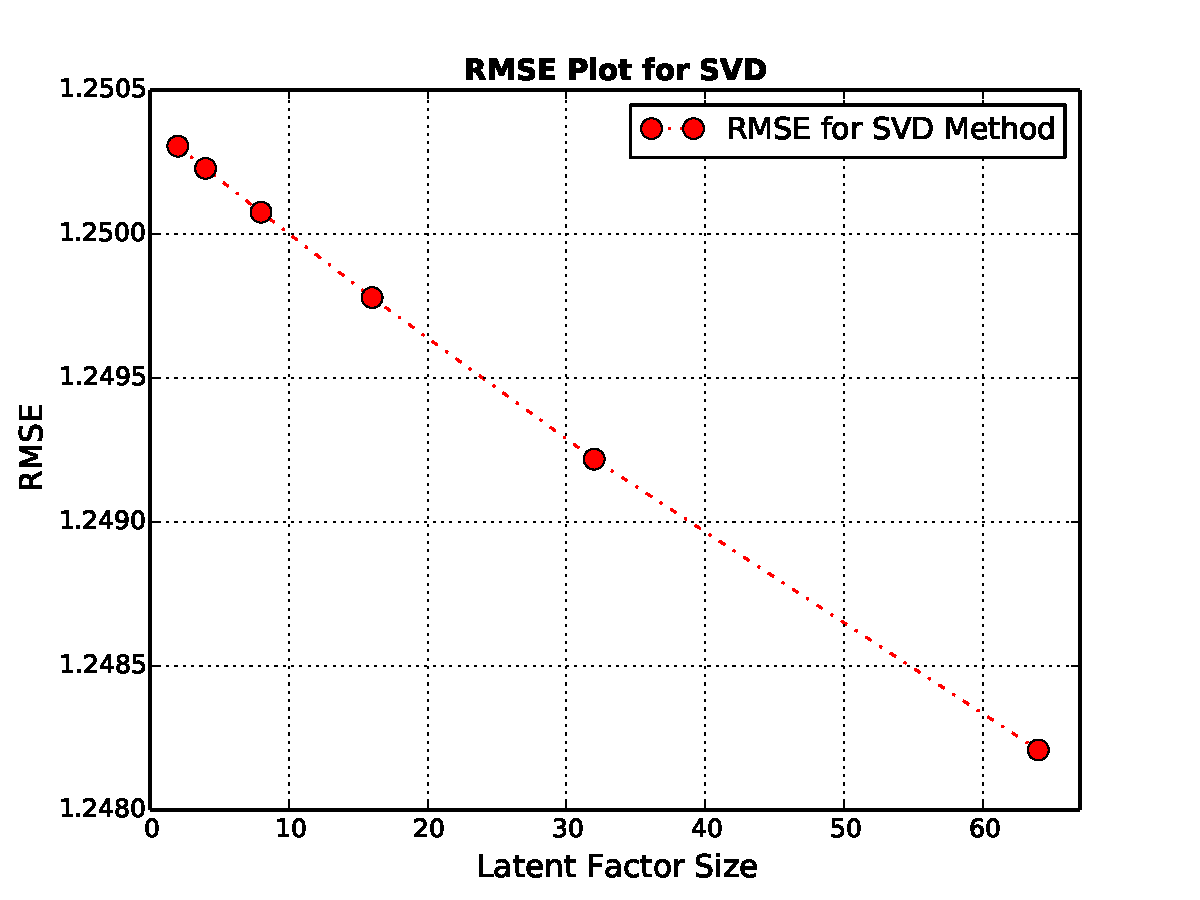
\includegraphics[scale=0.42]{Prj_images/SVD_RMSE.pdf} \end{center} 
	\begin{center}  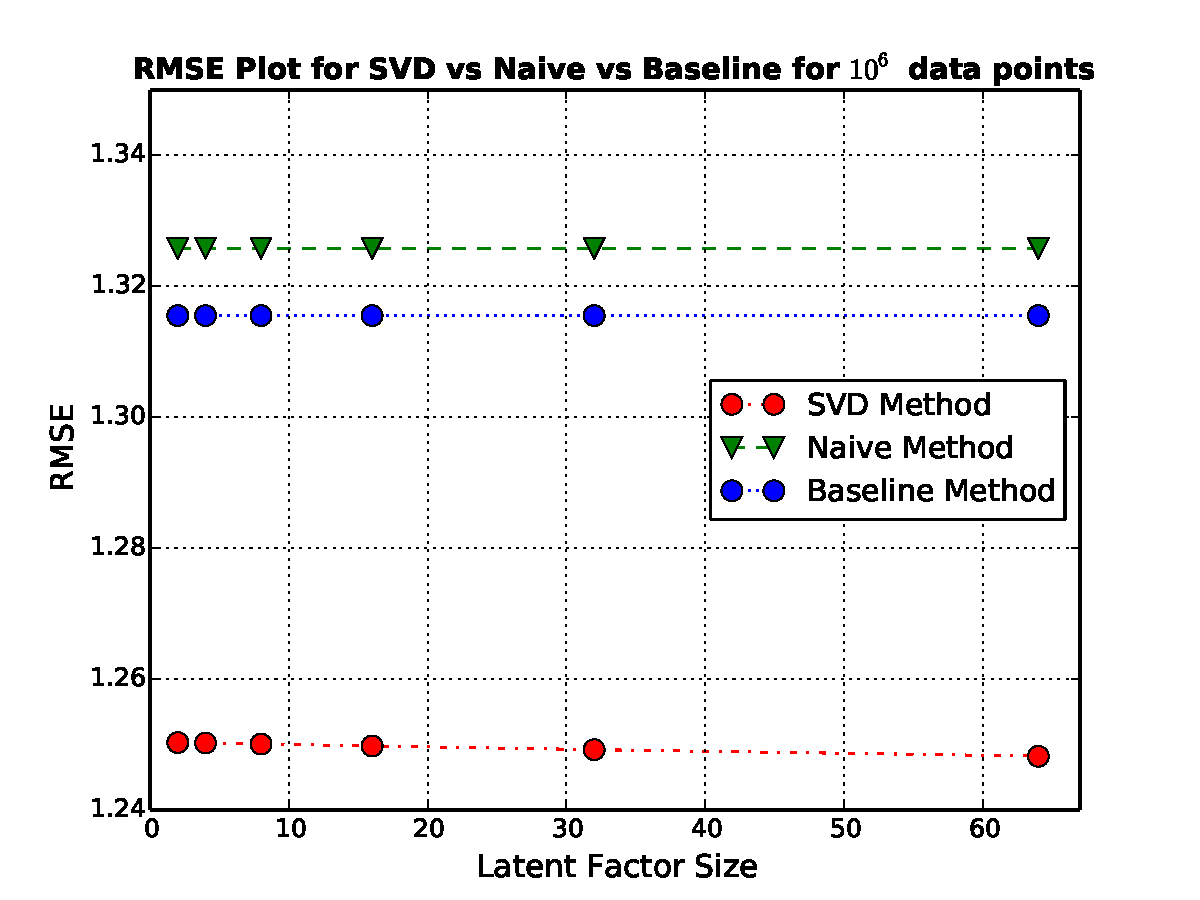
\includegraphics[scale=0.42]{Prj_images/All.pdf} \end{center} 

\section{Results}
	We consider our results to be relatively accurate since the RMSE obtained by running the algorithm on the complete dataset is significantly lower than the RMSE obtained by the simpler methods similar to what we can observe in \cite{koren2008factorization}. Moreover, the RMSE decreases as the number of latent factors in the model increases. Also, we notice that as we increase the number of latent factors the runtime of our program increases in a linear fashion. In the graph below we include the runtime measures for $2,4,8,16$ factors using an Intel Core i7-5600U running at $2.6$ GHz:
	
	\begin{center}  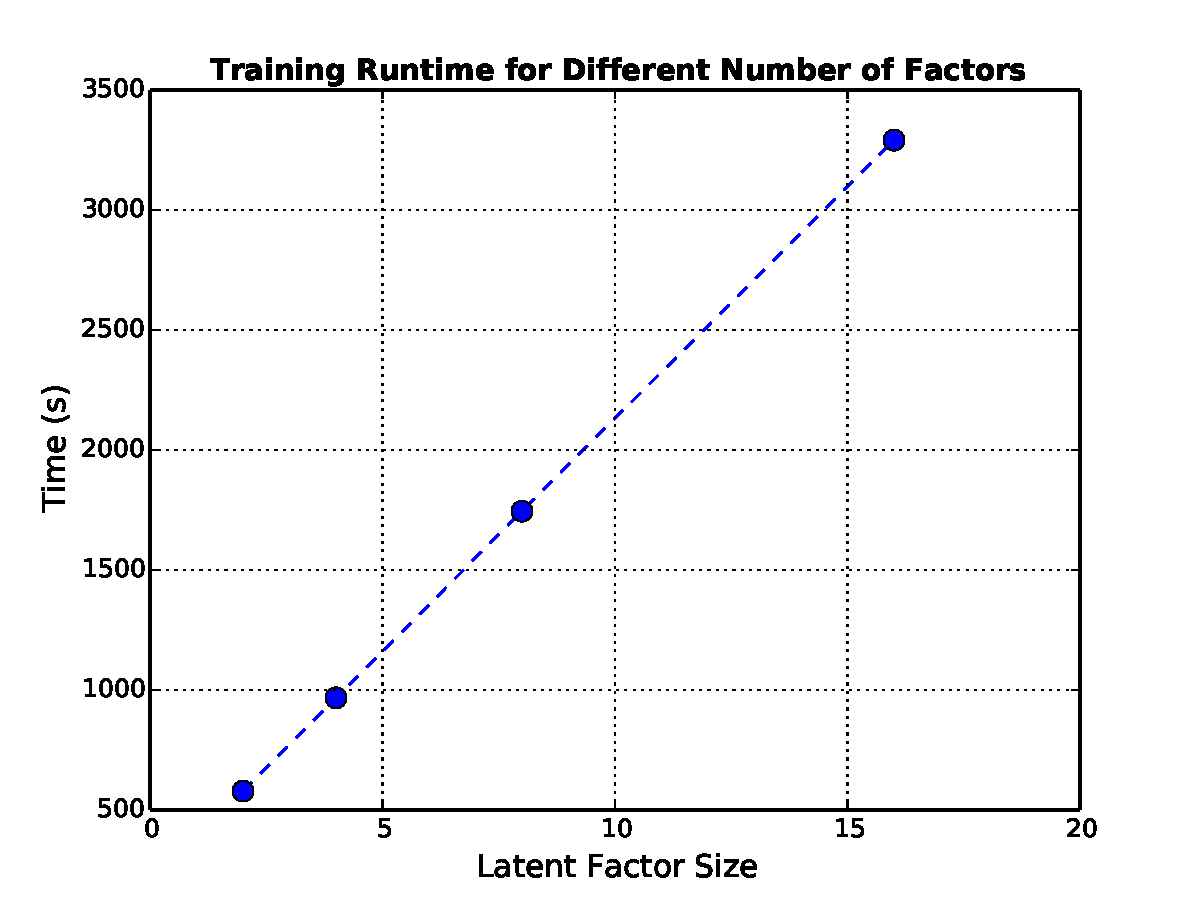
\includegraphics[scale=0.42]{Prj_images/runtime.pdf} \end{center}
	
	To test our implementation we recommend restaurants for user with id \texttt{PUFPaY9KxDAcGqfsorJp3Q} using 64 factors. The 
	restaurants as well as the rating predictions for this user are in Table \ref{tab_ratings}.
		\begin{table}[ht]
		\caption{Restaurants and Ratings}
		\vspace{0.3cm}
		\centering
		\begin{tabular}{c c c }
		\hline\hline
		Restaurant & Predicted Rating & Yelp Rating \\ [0.5ex] % inserts table %heading
		\hline 
		Waldsch\"anke & 5.00 & 5\\
		Green Traiteur \& Cafe &  4.93 & 5 \\
		XO Cafe \& Lounge & 4.90 & 3 \\
		Roly Poly  & 4.90 & 3.5\\
		Asia Food  & 4.87 & 4.5 \\
		
		%\\ [1ex]
		\hline
		\end{tabular}\\[0.5cm]
		\label{tab_ratings}
		\end{table}

		It is worth noticing that the recommended restaurants include ones with a lower rating on Yelp which suggests that 
		our recommender indeed gives personalized results for each user. Our algorithm does not naively suggest only top rated 
		restaurants. 

\section{Challenges}
	The main challenge that we faced was mainly to overcome the difficulty of working with all the data. At first, in order to narrow the 		problem down, we created two different files with 10,000 and 100,000 ratings respectively. Even in that case, it would take our algorithm 	more than an hour to terminate. As a result, we had to change our implementation approach and we were forced to work with a ratings matrix 	instead of using json files. Due to the structure of the Yelp Data, the ratings were very sparse therefore we chose to implement a Python 	sparse matrix in the coordinate (COO) format. We are able to run the program for all the data in roughly two hours for 16 factors. It is 	obvious that when we increase the number of factors the running time of the program increases. In order to be able to use more factors, 	we have to improve our running time. So our challenge now is to improve the running time so that we can increase the number of latent
	factors. Moreover, it would be helpful to extract the location of the user for whom the recommendation is performed so as to be able to 	recommend nearby restaurants. 	
\bibliographystyle{abbrv}
\bibliography{bibliography}
% In the unusual situation where you want a paper to appear in the
% references without citing it in the main text, use \nocite

%
%\bibliography{example_paper}
%\bibliographystyle{icml2015}

\end{document} 


% This document was modified from the file originally made available by
% Pat Langley and Andrea Danyluk for ICML-2K. This version was
% created by Lise Getoor and Tobias Scheffer, it was slightly modified  
% from the 2010 version by Thorsten Joachims & Johannes Fuernkranz, 
% slightly modified from the 2009 version by Kiri Wagstaff and 
% Sam Roweis's 2008 version, which is slightly modified from 
% Prasad Tadepalli's 2007 version which is a lightly 
% changed version of the previous year's version by Andrew Moore, 
% which was in turn edited from those of Kristian Kersting and 
% Codrina Lauth. Alex Smola contributed to the algorithmic style files.  
